\section{A Unified Framework for Salient Structure Detection by Contour-Guided Visual Search}

\begin{flushright}
    \author{
    Kai Fu Yang,
    Hui Li,
    Chao-Yi Li,
    and Young-Jie Li,
   \emph{Member}, 
    IEEE 
}
\end{flushright}

\begin{center}
    \emph{IEEE TRANSACTIONS ON IMAGE PROCESSING, VOL. 25, NO. 8, AUGUST 2016}
\end{center}

\subsection{INTRODUCTION}
In order to reduce the complexity in the analysis of a scene, a useful method 
is introduced to detect potential information, such as regions or 
objects, simultaneously. This method is called "\emph{Visual Saliency}". Before introducing
the topic, four types of concepts must be explained: (1)\emph{Fixations}: 
they concern the scene framed by the human eye. They are used to compare 
the methods of forecasting fixations. (2)\emph{ROI}: each region contains information, 
such as light or dark objects, which is intended to be separated.(3)\emph{Salient objects}: 
animals, people, cars etc. (4)\emph{Salient edges}: boundary of each object. The proposed 
method is based on carrying out a \emph{Salient Structure (SS) Detection},
useful for identifying the four previous properties, both in cluttered and 
simple scenes. The proposed framework is called \emph{CGVS (contour-guided visual 
search)}. This visual search tool identifies the targets using two types of 
paths: (1)\emph{selective path}: the boundaries of each object are detected, useful 
for estimating the position and size of the ROI: (2)\emph{non-selective path}: it 
can be properties such as color, luminary, texture etc. This search strategy 
carries out parallel processing on both paths, extracting global and local 
information. Finally, a Bayesian inference is applied to integrate the contour 
based spatial prior (CBSP), a useful method for extracting information on 
the boundaries, and local information in order to identify the salience of each 
pixel. 

\subsection{RELATED WORK}

\subsubsection{\emph{Fixation Prediction}}
Fixation prediction models aim to calculate salience maps, which are used to 
identify ROIs. Fixation prediction models provide smooth regions of interest 
rather than uniform regions that highlight all salient objects. These models 
only offer the ability to detect the position of potential objects while excluding 
other features such as surfaces or shapes, which are useful for object 
detection and recognition. The methods proposed to obtain a salience map 
are varied and range from the use of Bayesian Framework, to including those 
for machine learning. 

\subsubsection{\emph{Salient Object Detection}}
Existing methods, useful for extracting salient objects from a scene, rely on 
the contrast of the local or global region. Object detection is an operation 
related to the "object proposal" operation which attempts to generate a set 
of all objects in the scene, regardless of their salience. In this paper Bayesian 
inference is used to accomplish this task.

\subsubsection{\emph{Bridging the Two Tasks}}
Unlike the existing methods, the proposed one is able to obtain more detailed 
salient structures in terms of resolution, moreover it is able to operate in 
conditions in which the scene is simple or complex. Both tasks do not need 
specific tuning.

\subsection{CONTOUR-GUIDED VISUAL SEARCH MODEL}

\begin{figure}[htbp]
    \centering
    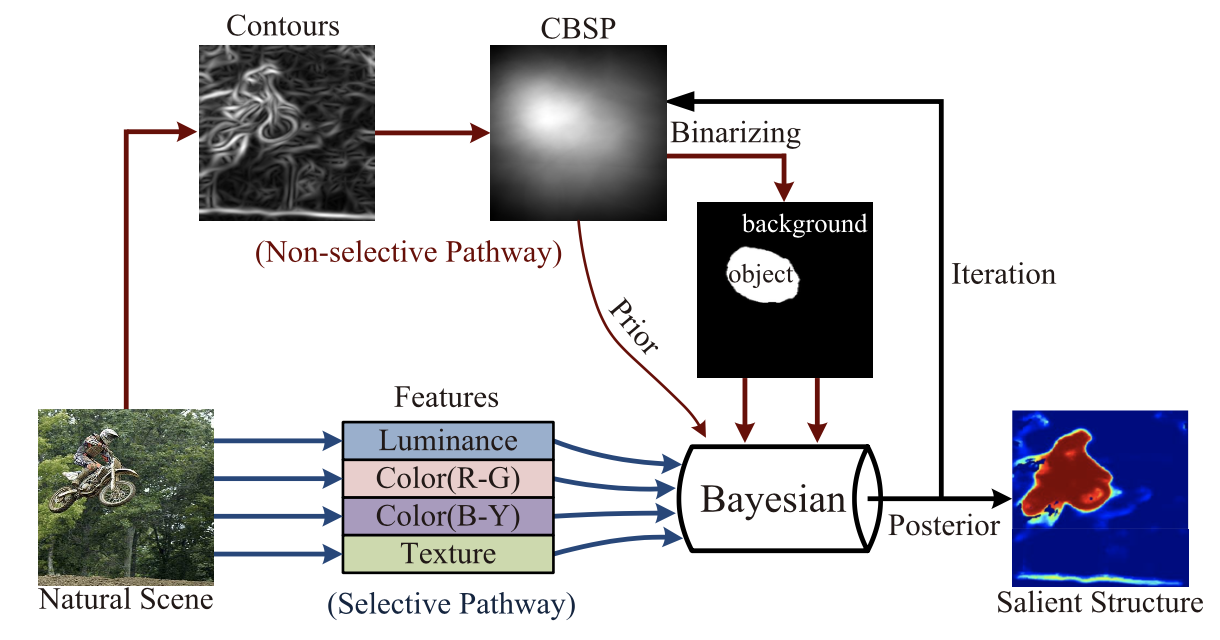
\includegraphics[width = 0.8\linewidth]{images/paper1/selective and non-selective pathways.png}
    \centering
    \caption{The flowchart of the porposed system}
    \label{fid: flowchart}
\end{figure}

The research of the possible potential positions, of the salient structures, is 
carried out with the help of the contour-based spatial prior (CBSP) process, 
which uses the contours detected in a non-selective path. At the same time, 
in the selective path, the local characteristics concerning color, luminance 
and texture are extracted. The information obtained from the CBSP is inserted 
into the Bayesian framework for the prediction of the salient structure. 
Finally, the output of the Bayesian framework will represent the salient structure 
which will be improved through an iterative procedure applied on the 
CBSP process. The flowchart of the proposed method is summarized in Fig. \ref{fid: flowchart}.

\subsubsection{\emph{Contour-Based Spatial Prior (CBSP)}}
\begin{figure}[htbp]
    \centering
    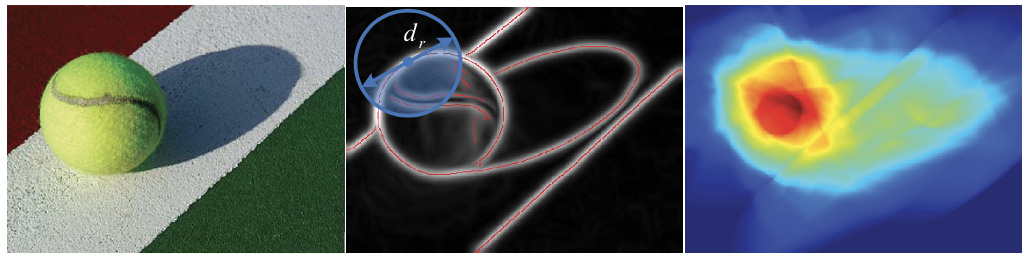
\includegraphics[width = 0.8\linewidth]{images/paper1/CBSP.png}
    \centering
    \caption{CBSP reconstruction}
    \label{fid: CBSP}
\end{figure}
Within the non-selective path, the crucial operation is to calculate the 
approximate spatial weights of salience based on the distribution of the previously 
detected contours. In this path there is the problem of determining 
the local information of each object. The solution to the problem is based 
on an operation that fills the regions delimited by these contours. A very 
efficient method proposed in \cite{0747815500} result is used for the extraction of the contours.
An example of CBSP reconstruction is shown in Fig. \ref{fid: CBSP}. Each pixel 
has a direction represented by a radius $ d_r $ which is equal to $d_r = min (H, W) / 3$, where 
\emph{H} and \emph{W} correspondingly indicate the width and height of the entire image.
The diameter divides the circle into two parts where, on each of these, for 
each pixel belonging to the edge, the average response of the edge (AER) will 
be calculated. This calculation is useful in deciding which of the two halves 
will belong to the salient region. Each spatial weight of salience is denoted 
by $ S_e $, while the added bias is denoted by $ S_c $ and both are normalized in the 
range of [0,1]. The value, which in turn will be normalized, of CBSP is given by: $$ S_w = S_e + S_c $$

\subsubsection{Low-Level Feature Extraction}
Features such as color (rgb), luminance (flum) and texture are extracted in 
parallel. There are complicated regions in a texture that can be represented. 
For this purpose, the texture channel ($ {f_{ed}} $)  has been introduced, which is 
useful to better represent the salient regions using the contour density (ED). 
The texture channel is calculated by using an 11x11 filter that smooths the 
edges.

\subsubsection{Bayesian Inference With Contour Guidance}
Bayesian inference gives the possibility to calculate the probability that a 
pixel x may belong to a salient structure s. This probability is computed as:
$$ p(s|x) = \frac{p(s)p(x|s)}{p(s)p(x|s)+p(b)p(x|b) } $$
Where $ p(x|s) $ is the probability of a pixel belonging to a salient structure, 
$ p(x|b) $ is the probability that a pixel belongs to the background, $ p(b)=1-p(s) $,
finally $ p(s)=Sw $ represents the CBSP value. The implementation 
details are as follows.
\begin{enumerate}
    \item \emph{Predict the size of Potential Structure}: this procedure, through a binarization of the map obtained 
    from $ p(s) $, separates the salient structures from the background, all 
    through the use of a threshold. This threshold is calculated using the 
    local parameters (color, luminance, etc.), a percentage not greater than 
    50\% useful to denote the size of the salient structure, an initial weight 
    and finally two sets of pixels corresponding to the background and the 
    foreground (salient structure).
    \item \emph{Evaluate the Importance of Each Feature}: a feature is considered important 
    when the difference between the average pixel values of its 
    salient structure and those of the background is large enough, i.e. when \emph{$ w_i $} 
    takes on a satisfiable value.
    \item \emph{Calculate the Observation Likelihood}:in order to calculate the observed 
    probabilities, the different color channels \emph{($ f_{lum}, f_{rg}, f_{by}, f_{ed} $)} are used, 
    and the distribution functions $ p(x_i | S_{T_{opt}}) $ and $ p(x_i | B_{T_{opt}}) $ where $ S_{T_{opt}} $ 
    represents the set of pixels belonging to the structure salient, while 
    $ B_{T_{opt}} $ represents the set of pixels belonging to the background.
    $$ p(x|s) = \prod_{i \in {\{} f_{lum}, f_{rg}, f_{by}, f_{ed} {\}}} {(p(x_i | S_{T_{opt}}))^{w_i}} $$
    $$ p(x|b) = \prod_{i \in {\{} f_{lum}, f_{rg}, f_{by}, f_{ed} {\}}} {(p(x_i | B_{T_{opt}}))^{w_i}} $$
    \item \emph{Enhance the Salient Structure by Iterating}: the salient structures, at 
    each instant \emph{t}, with $ t = t_0,…, t_n $, are iteratively improved by applying 
    a median filter on each of them. In addition, the weight attributed to 
    the importance of each feature is changed. Finally, the CGVS model 
    will operate on a set of instants \emph{t}, thus forming the contour-guided 
    visual search.
\end{enumerate}

\subsection{EXPERIMENTS}
The proposed method was evaluated on different datasets. For the fixation 
prediction the datasets are \cite{0747815530} \cite{0747815531} \cite{0747815579}, while for the salient object detection \cite{0747815506} \cite{0747815508} \cite{0747815518}.

\subsubsection{\emph{Basic Property of the Proposed Model}}
The proposed system allows to carry out a multiple search of objects. In 
comparison to the work of Itti et al. \cite{0747815505} the proposed system is able to detect, 
after several iterations, the region and therefore the salient object.

\subsubsection{\emph{Fixation Prediction}}
The prediction of fixation indicates the likelihood with which a human is 
looking at a given position in the scene. There are several metrics that are 
used to evaluate the prediction such as Natural Scanpath Saliency (NSS) 
and ROC (AUC). In the following article the ROC method is mainly used, 
on three types of datasets, to compare the proposed system with o already 
existing at the state of the art, as shown in Fig. \ref{fig: ROC}.
\begin{figure}[htbp]
    \centering
    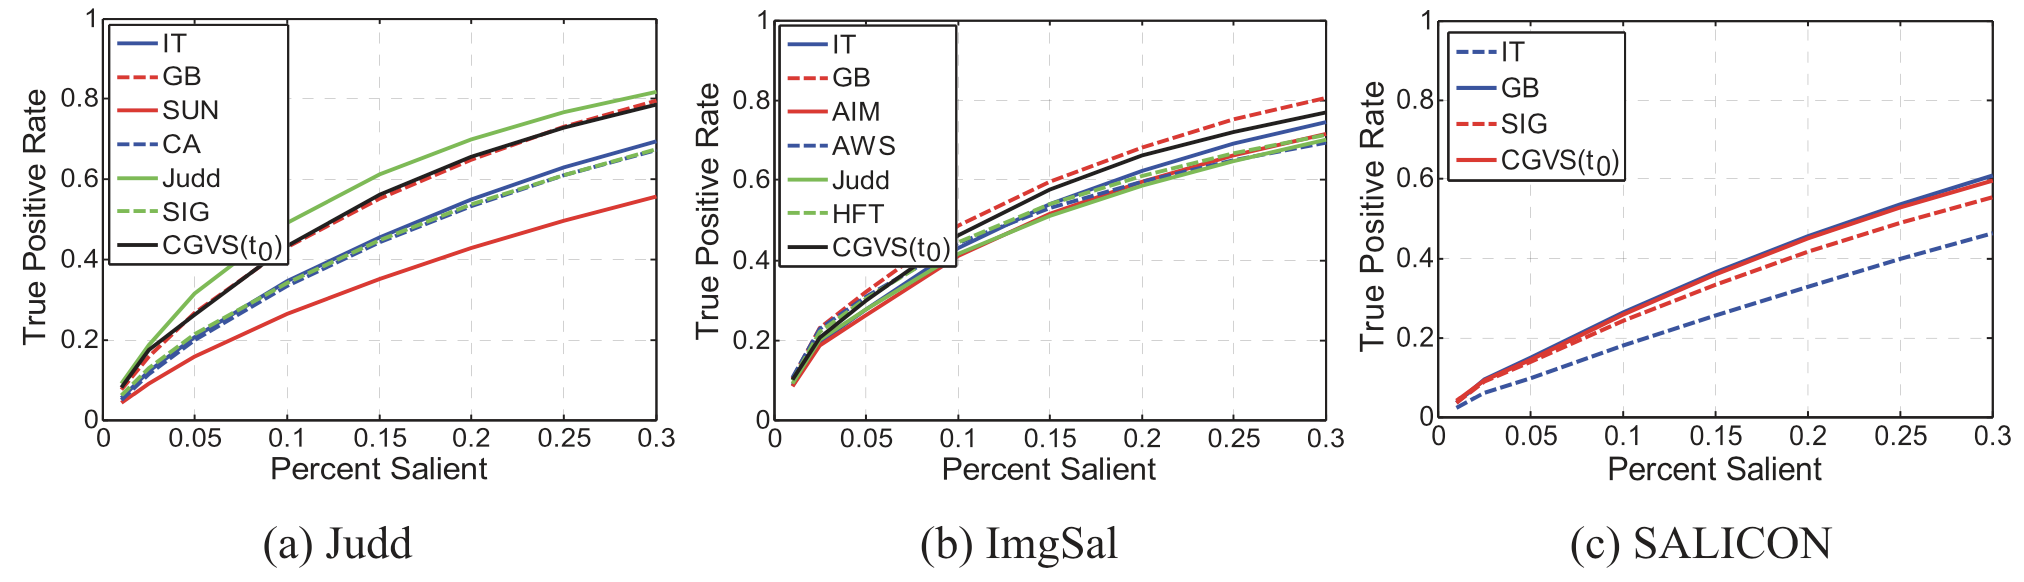
\includegraphics[width = 1 \linewidth]{images/paper1/ROC.png}
    \centering
    \caption{ROC comparison}
    \label{fig: ROC}
\end{figure}

Several proposed methods, such as the CA \cite{0747815502}, in order to increase the ROC 
index, aim to have a first fixation that is limited to having a central prior 
in the scene. On the other hand, this method will lose information on surrounding 
objects. In the proposed method, the computation of the CBSP 
takes into account this center prior, without however losing the information 
on the other objects in the scene.

\subsubsection{\emph{Salient Object Detection}}
\begin{figure}[htbp]
    \centering
    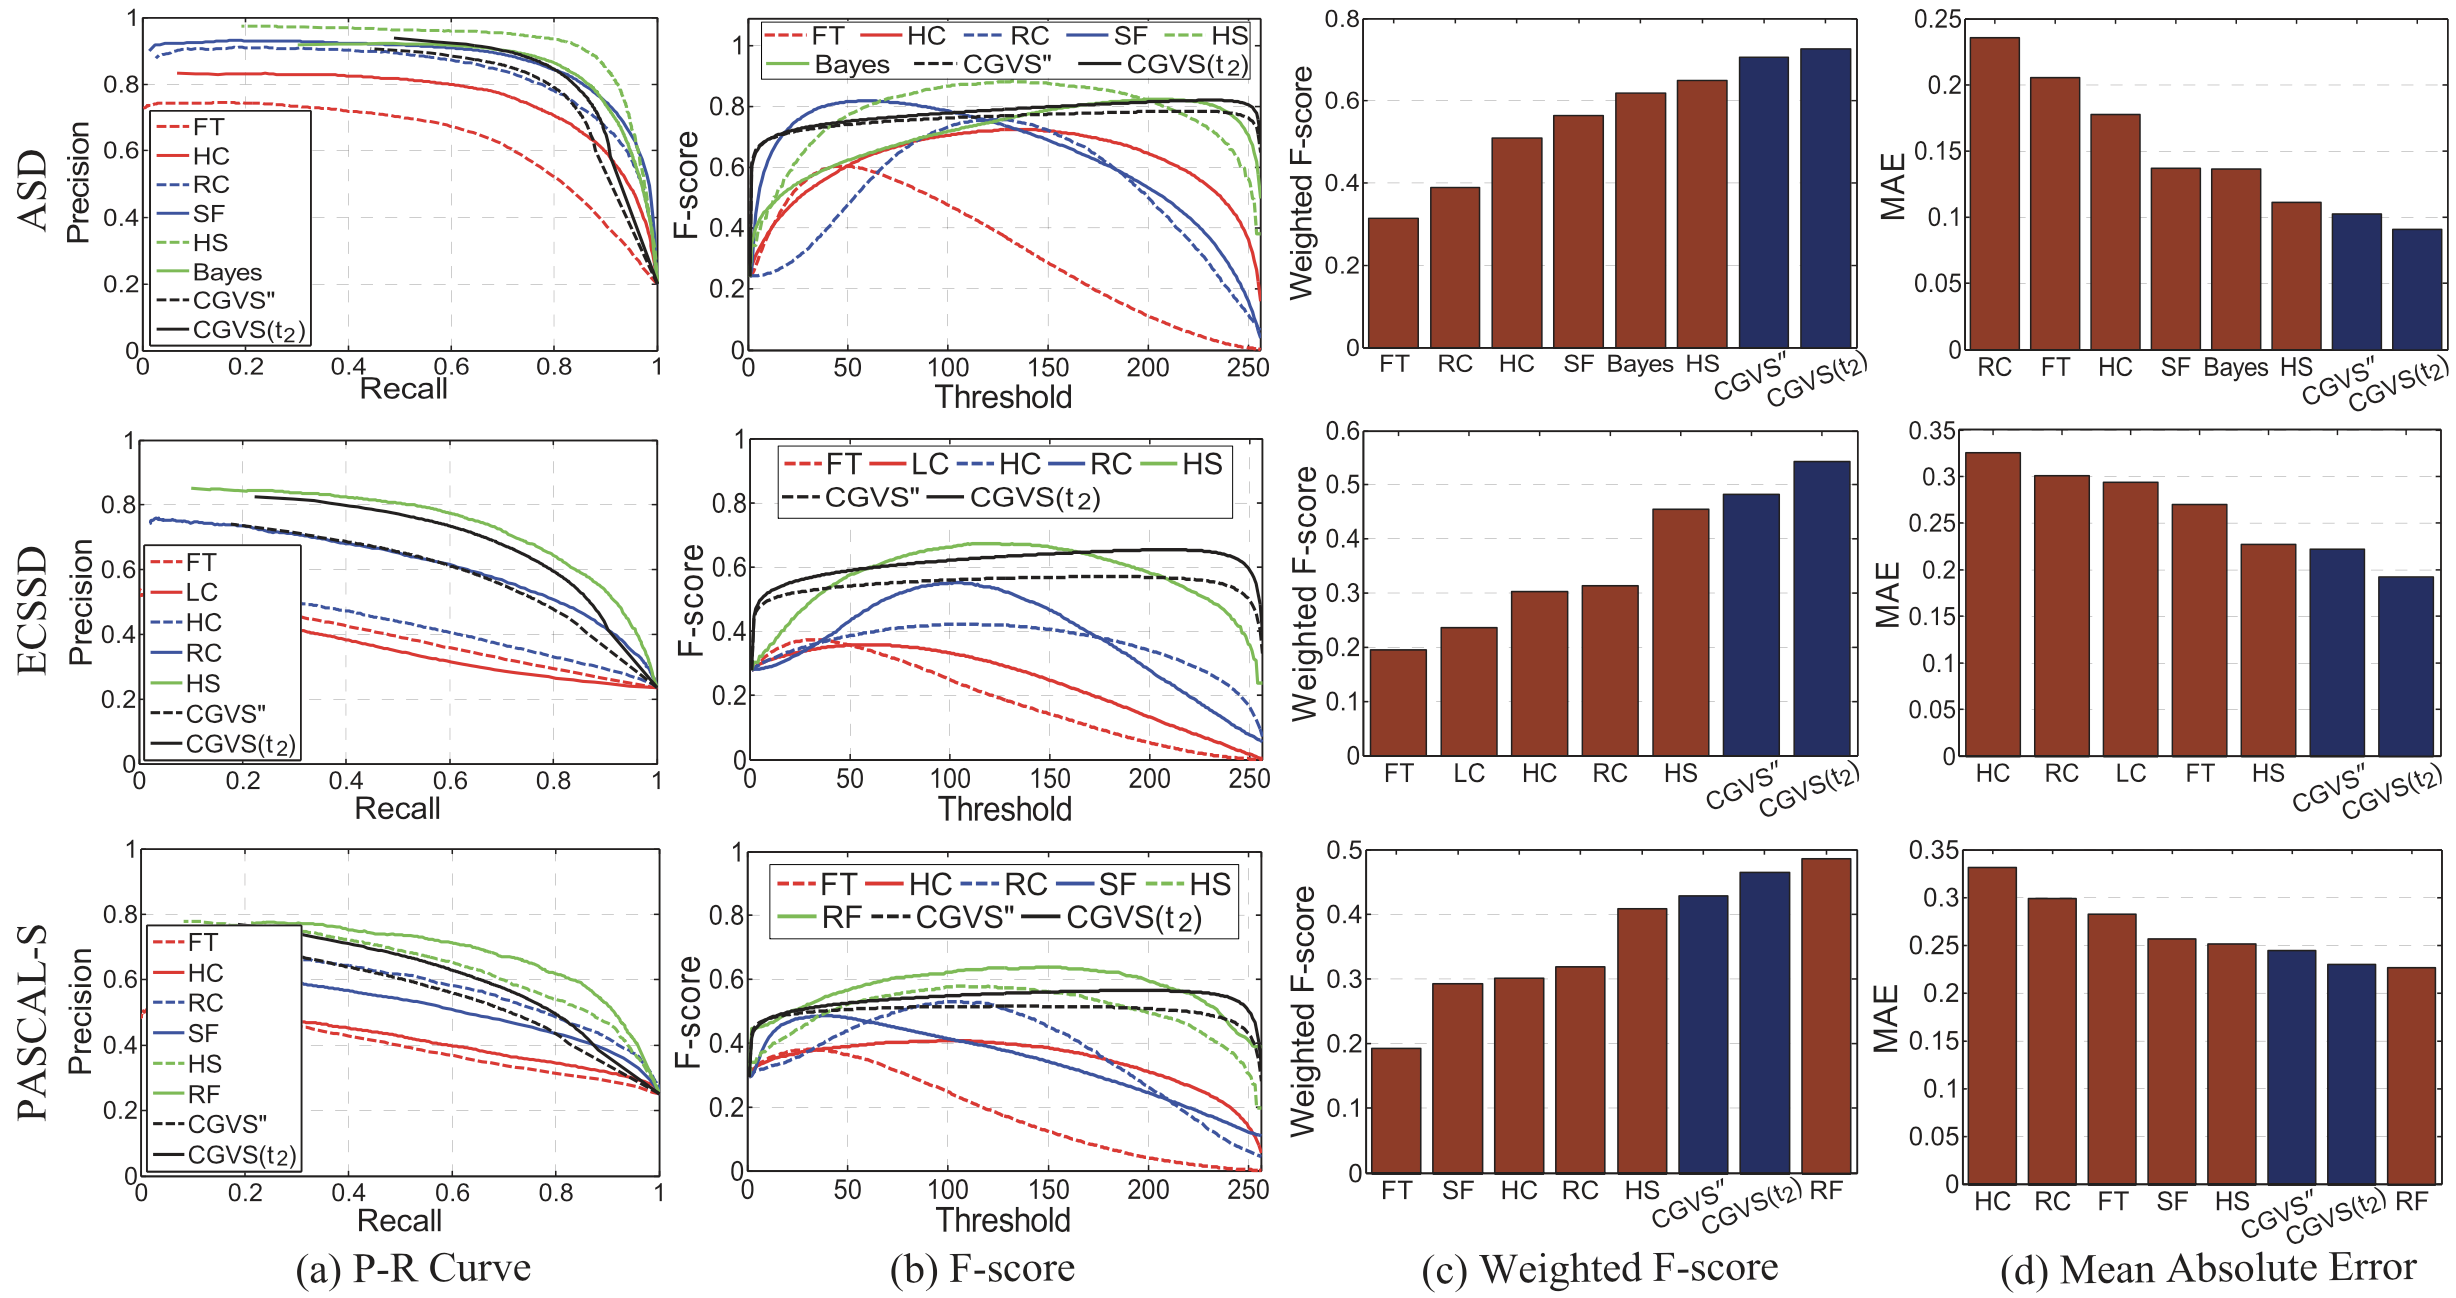
\includegraphics[width = 1 \linewidth]{images/paper1/metrics.png}
    \centering
    \caption{Metrics comparison}
    \label{fig: metrics}
\end{figure}
To compare the performance of the salient object detection, metrics such 
as Precision, Recall, F-score, Weighted F-score and MAE (Mean Absolute 
Error) were used on three types of datasets (ASD, ECSSD, PASCALS). The 
results showed that for the first two metrics (P-R), systems such as HS and 
RF are the best, while for the F-score the proposed method is able to consider 
a greater range of thresholds. As it can be seen, in these two metrics the 
proposed system (\emph{CGVS($ t_2 $)}) considers the central bias unlike the others. 
If the central bias were not considered, the results decrease but are still 
satisfactory (\emph{CGVS''}). However, in the remaining two metrics, the proposed 
system is the best, except in the PASCALS dataset where the best is the RF 
method.

\subsubsection{\emph{Between Saliency Map and Salient Object}}
Most fixation prediction methods perform poorly when used to detect salient 
objects. To solve this problem, a two-dimensional Gaussian distribution is 
applied to each salience map derived from any method. The derived output 
will be used as an initial CBSP from which the salient objects can be 
extracted with the previously proposed calculations. The metrics, used to 
measure the performance of the different methods, improve if the methods 
replace their salience map with CBSP.

\subsubsection{\emph{Extended Saliency-Related Applications}}
The peculiarity of the proposed method also lies in the search for salient 
edges. This process is possible by replacing the four color components with 
three luminance gradients and two color-opponent channels. The system also 
proves to be capable of being able to detect text as well.